\graphicspath{{./figures/}}
\chapter{Implementation}
This chapter focuses on the overall project's implementation.
It mainly covers the four parts hardware assembly, long jump analysis,
drone control and their consolidation into one \ac{GUI}.

\section{Hardware}\label{sec:4_hardware}
In order to capture high-quality video recordings that cover a complete long 
jump, from the first step all the way to the landing, a drone is used to fly
next to the athlete throughout the whole process.
Thus, a drone in form of a quadcopter is built from scratch.
Its control will be integrated seamlessly in the projects' \ac{GUI}.\\
This section introduces the hardware components that are used for building 
this drone as well as its flight control unit.\\
A short outline of the hardware is given in.
The assembly is shown in, while ... focuses on the PixHawk flight 
controller and its setup.

\subsection{Hardware selection}\label{subsec:4_hardware_selection}
Currently, commercial drone hardware on the market is mainly separable into 
the two large areas of fully remote controlled \ac{FPV} hardware and hardware 
for (autonomous) drones that can usually carry more load, e.g.~heavy cameras.
Even though the quadcopter in this project needs to be remotely 
controllable from a ground station pc, it is still more likely to be located 
in the latter one.\\
Generally the hardware was chosen based on the following criteria:
\begin{itemize}
    \item price
    \item compatibility
    \item size
\end{itemize}

\subsection*{Flight Hardware}\label{subsec:4_filght_hardware}
The main hardware that a quadcopter needs to fly will, in the following, be
referred to as \textit{flight hardware}.
This includes frame, motors, rotors, \acp{ESC} and a \ac{PDB}.\\
The main platform on which all drone hardware is mounted, is referred to as
a quadcopter's frame.
As this project's drone does not need to carry any heavy load, such as high 
precision camera systems or other sensors, a rather compact frame would 
theoretically be sufficient.
However, compact frames tend to be less stable compared to larger frame sizes 
which could lead to a lower video recording quality and thus require more 
complex post-processing software.
Moreover, the assembly process on larger frames is more convenient and 
replacing parts is easier.
Additionally, compact frames are most commonly used in areas that demand quick
reaction times for high speed flight maneuvers, e.g.~in drone racing.
This however is not needed in this project's context.\\
Taken the mentioned considerations into account the mid-sizes \textit{Holybro 
S500 V2} frame kit is chosen.
Besides the frame, the kit also includes a landing gear and rotors.
Moreover, the main platform includes a \ac{PDB} to split the battery's power 
equally to all four motors.\\
An overview of all included parts is given in \autoref{fig:4_frame_kit}.
\begin{figure}[!h]
    \centering
    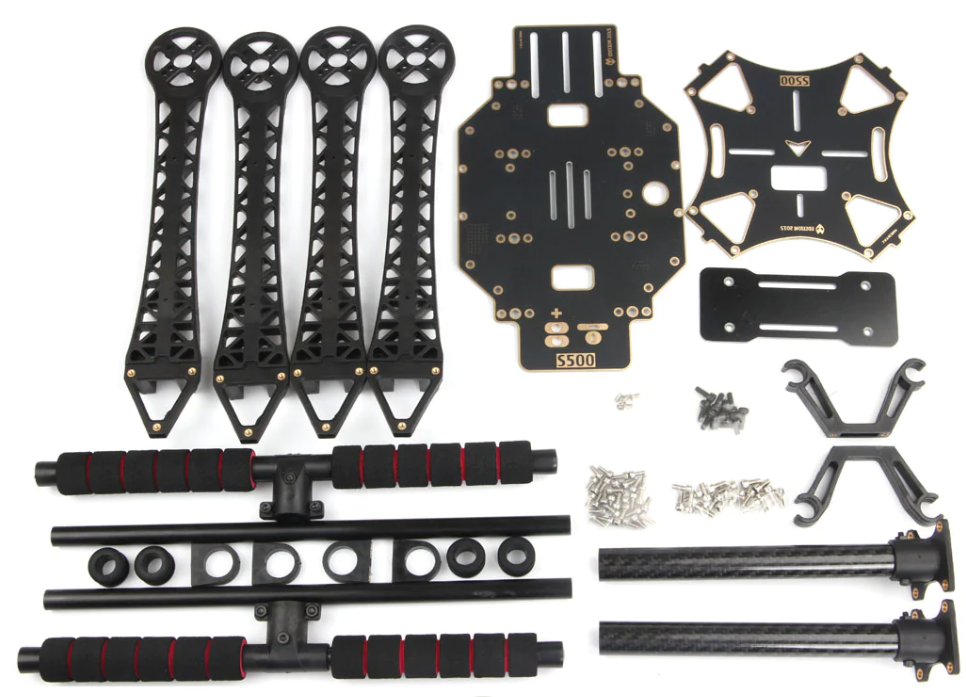
\includegraphics[scale=0.6]{frame-kit.png}
    \caption[Frame kit]{Holybro S500 V2 frame kit}
    \label{fig:4_frame_kit}
\end{figure}
\FloatBarrier
\noindent Besides the frame, motors and compatible \acp{ESC} are crucial 
flight hardware components.
Each motor requires an own \ac{ESC} that translates signals from a flight 
control unit to a voltage and thereby control the motors' rotation speed.
To guarantee compatibility, both components were chosen from Holybro as well
and can be seen in \autoref{fig:motors_and_esc}.
\begin{figure}[!h]
    \begin{subfigure}[b]{0.48\textwidth}
        \includegraphics*[scale=0.15]{motor.jpg}
        \caption{920KV Motor}
    \end{subfigure}
    \hfill
    \begin{subfigure}[b]{0.5\textwidth}
        \includegraphics*[scale=0.15]{esc.jpg}
        \caption{\acl*{ESC}}
    \end{subfigure}
    \caption[Motor and \acs*{ESC}]{Motor (a) and \acs*{ESC} (b)}
    \label{fig:motors_and_esc}
\end{figure}
\FloatBarrier

\subsection*{Control Hardware}\label{subsec:4_control_hardware}
As noted before, the \acp{ESC} which are directly connected to the motors
receive their input signals from a so-called \textit{flight control unit}. 
